\subsection{Projektstrukturplan}

Ein größeres Projekt umzusetzen erfordert viel Arbeit. Oftmals erscheinen Aufgaben so groß, als dass man nirgend wo starten kann. Um Arbeit und konkrete Arbeitsschritte besser darstellen zu können greifen Projektmanager oftmals auf den Projektstrukturplan zurück. Der Projektstrukturplan bricht größere und komplexere Arbeiten in kleine und konkrete Arbeitspakete. Die konkreten Arbeitspakete werden anschließend gruppiert, sequenziell nummeriert und den verschiedenen Abteilungen bzw. Arbeitern zugeteilt werden. Anhand eines Projektstrukturplans kann ein Gantt Plan erstellt werden. Der Gantt Plan zeigt die zeitliche Abfolge der einzelnen Arbeitspakete. Der Projektstrukturplan ist ein wichtiges Werkzeug für die Planung und Steuerung von Projekten. In Abbildung \ref{fig:projektstrukturplan} wird der Projektstrukturplan des Prototypen dargestellt.

\begin{figure}[H]
  \centering
  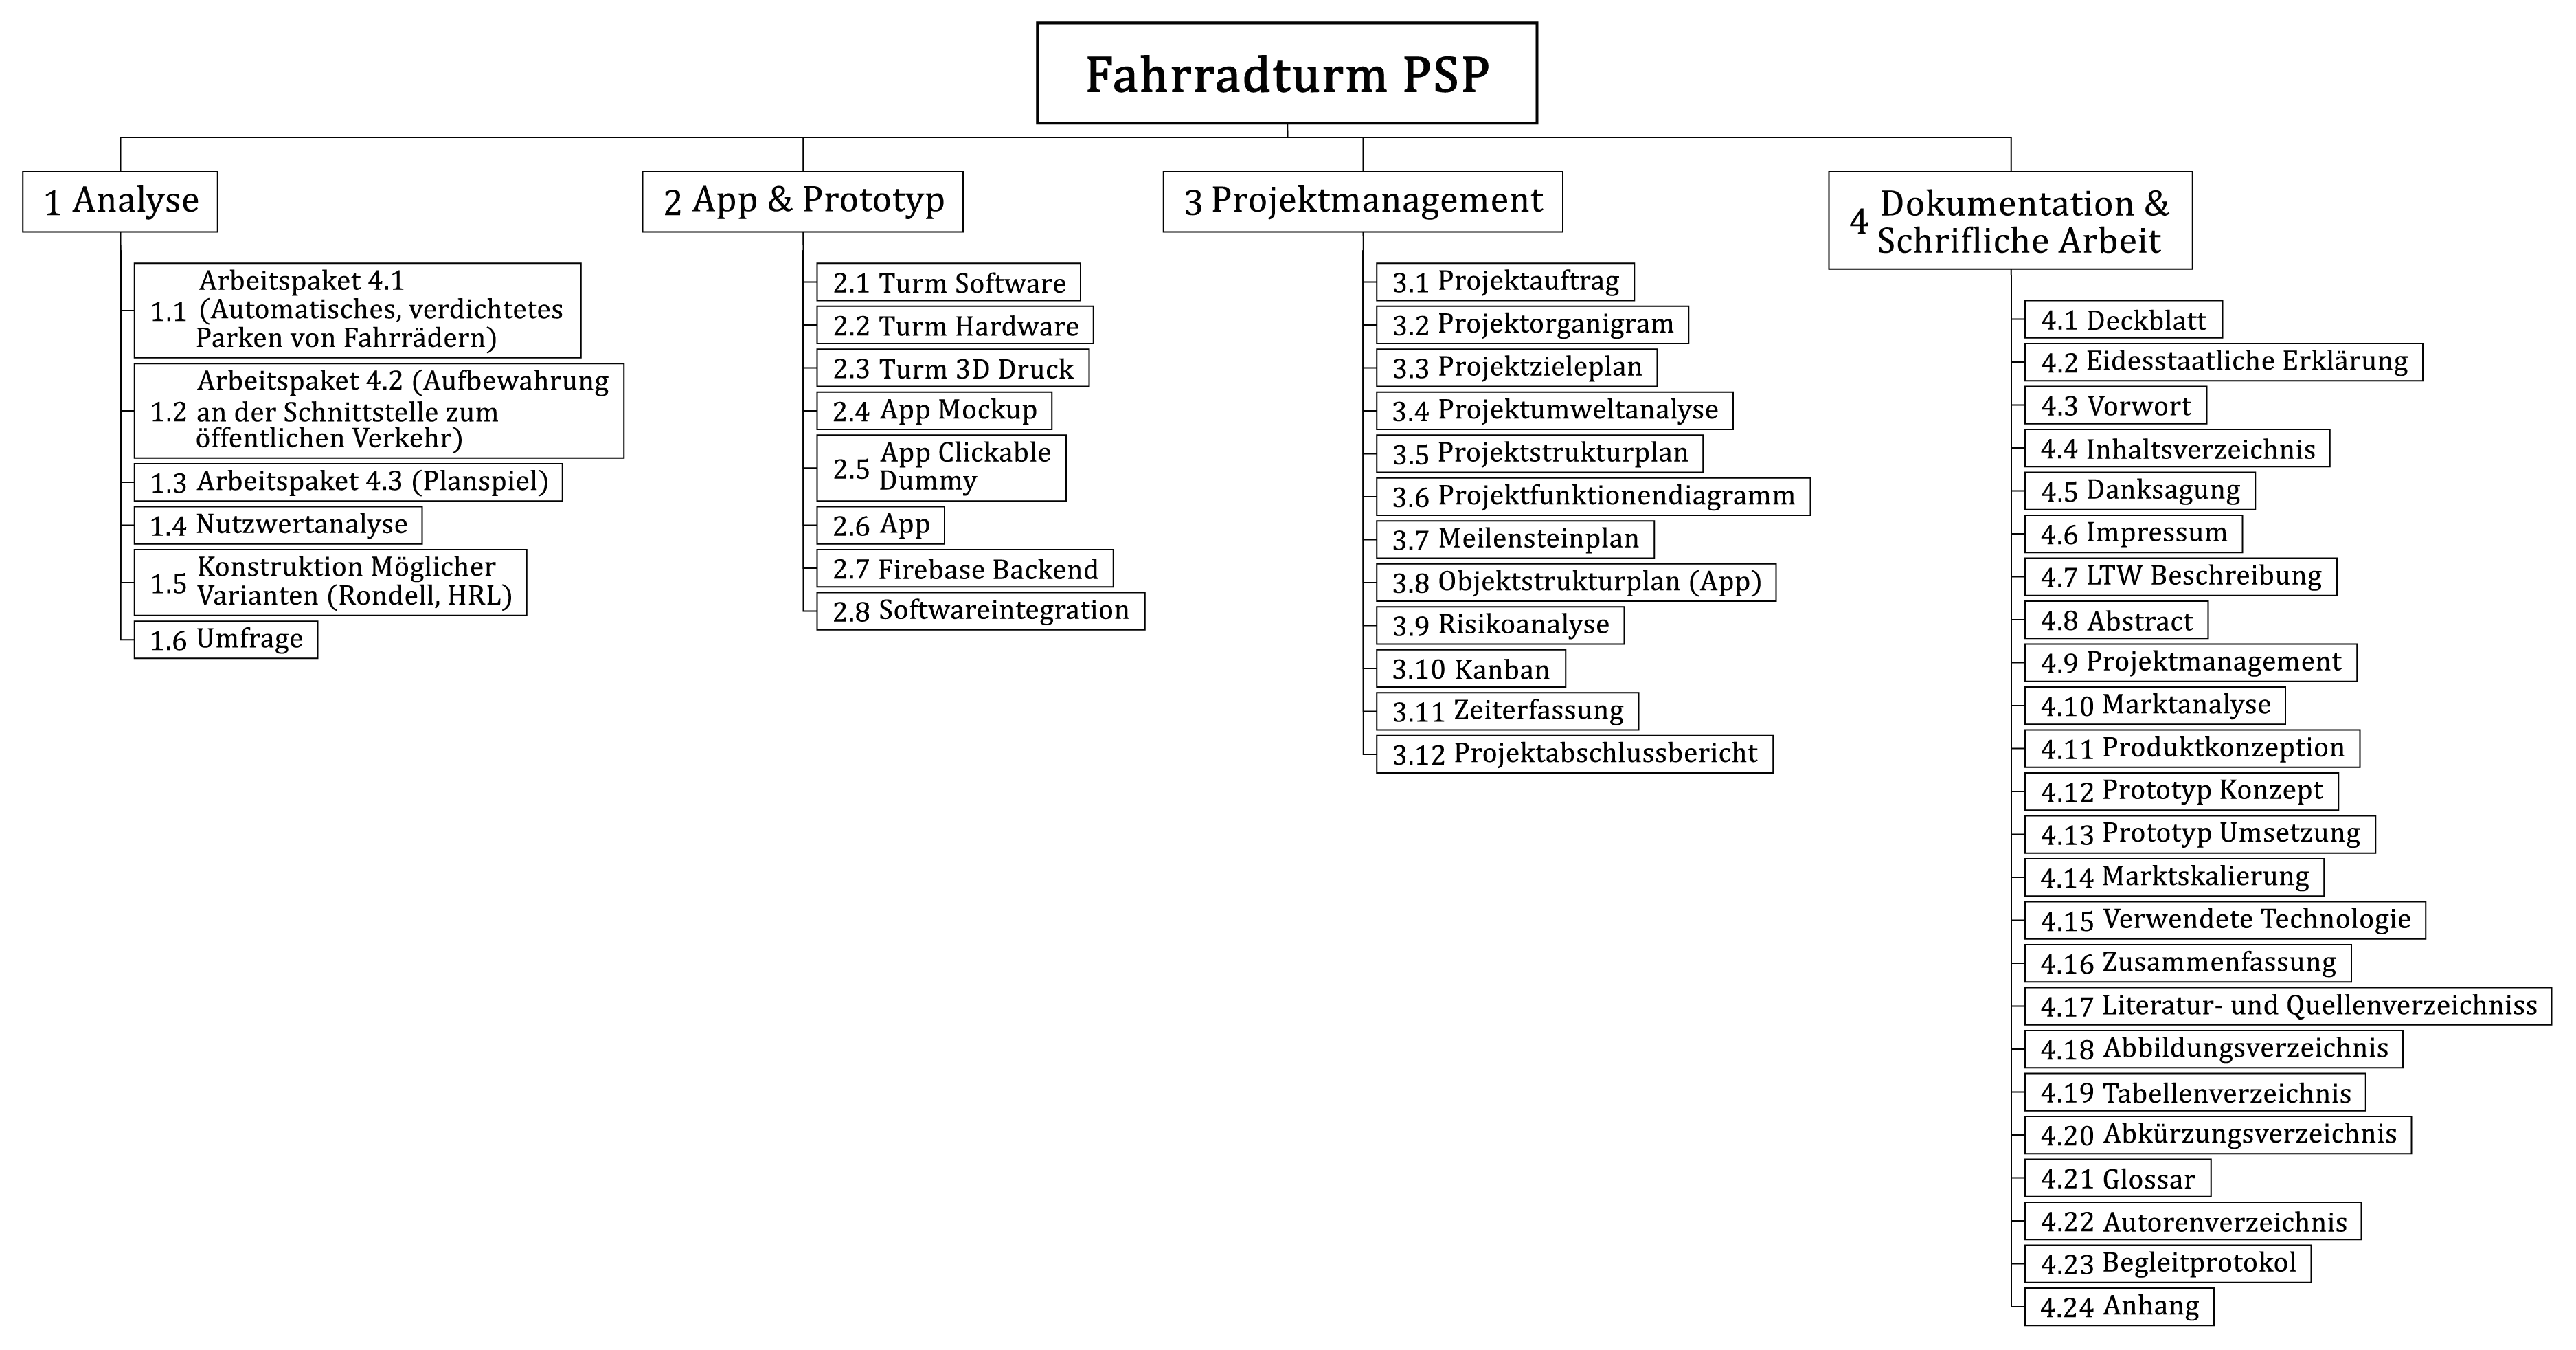
\includegraphics[width=1\textwidth]{images/projektstrukturplan}
  \caption{Projektstrukturplan}
  \label{fig:projektstrukturplan}
\end{figure}
